\documentclass[12pt,a4paper]{article}
\usepackage{amsmath}
\usepackage[english]{babel}
\usepackage{graphicx}
\usepackage{listings}
\usepackage{fullpage}
\usepackage[T1]{fontenc}
\usepackage{enumerate}
\usepackage[makeroom]{cancel}
\usepackage{hyperref}

\lstdefinestyle{custompython}{
  belowcaptionskip=1\baselineskip,
  breaklines=true,
  frame=L,
  xleftmargin=\parindent,
  language=bash,
  basicstyle=\footnotesize\ttfamily,
  showstringspaces=false,
  %commentstyle=\itshape\color{purple!40!black},
  %keywordstyle=\itshape\color{green!40!black},
  %identifierstyle=\color{blue},
  %stringstyle=\color{orange},
}

\author{
  Cheng, Lidens\\
  \texttt{lidenscheng@email.arizona.edu}
  \and
  McClintock, Tom\\
  \texttt{tmcclintock@email.arizona.edu}
  \and
  Wagoner, Erika\\
  \texttt{wagoner47@email.arizona.edu}
}
\title{Astr 513: Homework 2}

\begin{document}
\maketitle
  
\section{Parts A and B}

\begin{enumerate}[a)]
 \item We can use three kinematic equations to find $u_x$ and $u_y$ in terms of $R$, $g$, and $h$:
 \begin{enumerate}[(1)]
  \item $0 = u_y^2 - 2 g h \Rightarrow \boxed{u_y = \sqrt{2 g h}}$
  \item $0 = u_y - \frac{g t}{2} = \sqrt{2 g h} - \frac{g t}{2} \Rightarrow t = \sqrt{\frac{8 h}{g}}$
  \item $R = u_x t = u_x \sqrt{\frac{8 h}{6}} \Rightarrow \boxed{u_x = R \sqrt{\frac{g}{8h}}}$
 \end{enumerate}
 In the error propagation method, the expected values for $u_x$ and $u_y$ are just the values $u_x^0$ and $u_y^0$ we obtain when we insert the mean values $R_0$, $g_0$, and $h_0$ into the expressions above:
 \begin{subequations}
  \begin{align*}
   u_x^0 &= R_0 \sqrt{\frac{g}{8 h}} \\
   &= 10.0 \mathrm{m} \sqrt{\frac{9.81 \cancel{\mathrm{m}} \cdot \mathrm{s}^{-2}}{8 \cdot 1.0 \cancel{\mathrm{m}}}}
  \end{align*}
  \begin{equation}
   \boxed{u_x^0 \approx 11.1 \mathrm{m} \cdot \mathrm{s}^{-1}}
  \end{equation}
 \end{subequations}
 \begin{subequations}
  \begin{align*}
   u_y^0 &= \sqrt{2 g_0 h_0} \\
   &= \sqrt{2 \cdot 9.81 \mathrm{m} \cdot \mathrm{s}^{-2} \cdot 1.0 \mathrm{m}}
  \end{align*}
  \begin{equation}
   \boxed{u_y^0 \approx 4.43 \mathrm{m} \cdot \mathrm{s}^{-1}}
  \end{equation}
 \end{subequations}
 
 When using propagation of errors, the fractional error on some function $f\left(\vec{x}\right)$ with mean $\vec{x}$ values $\vec{x}^0$ and errors $\sigma_i$ can be found by $\frac{\sigma_f}{f} = \sqrt{\displaystyle \sum_{i = 1}^n \left(\frac{\partial \ln f}{\partial x_i}\right)_{\vec{x}^0} \sigma_i^2 }$. So we first take the natural log of $u_x$ and $u_y$:
 \begin{align*}
  \ln u_x &= \ln R + \frac{1}{2} \ln g - \frac{1}{2} \ln h - \frac{3}{2} \ln 2 \\
  \ln u_y &= \ln 2 + \ln g + \ln h
 \end{align*}
 Then we find that
 \begin{subequations}
  \begin{align*}
   \frac{\sigma_{u_x}}{u_x} &= \sqrt{\left(\frac{\sigma_R}{R_0}\right)^2 + \frac{1}{4} \left(\frac{\sigma_g}{g_0}\right)^2 + \frac{1}{4} \left(\frac{\sigma_h}{h_0}\right)^2} \\
   &= \sqrt{\left(\frac{0.2\cancel{\mathrm{m}}}{10.0\cancel{\mathrm{m}}}\right)^2 + \frac{1}{4} \left(\frac{0.05 \cancel{\mathrm{m}} \cdot \cancel{\mathrm{s}^{-2}}}{9.81 \cancel{\mathrm{m}} \cdot \cancel{\mathrm{s}^{-2}}}\right)^2 + \frac{1}{4} \left(\frac{0.2 \cancel{\mathrm{m}}}{1.0 \cancel{\mathrm{m}}}\right)^2}
  \end{align*}
  \begin{equation}
   \boxed{\frac{\sigma_{u_x}}{u_x} \approx 0.10}
  \end{equation}
 \end{subequations}
 for $\sigma_{u_x}$, and for $\sigma_{u_y}$,
 \begin{subequations}
  \begin{align*}
   \frac{\sigma_{u_y}}{u_y} &= \sqrt{\frac{1}{4} \left(\frac{\sigma_g}{g_0}\right)^2 + \frac{1}{4} \left(\frac{\sigma_h}{h_0}\right)^2} \\
   &= \frac{1}{2} \sqrt{\left(\frac{0.05 \cancel{\mathrm{m}} \cdot \cancel{\mathrm{s}^{-2}}}{9.81 \cancel{\mathrm{m}} \cdot \cancel{\mathrm{s}^{-2}}}\right)^2 + \left(\frac{0.2 \cancel{\mathrm{m}}}{1.0 \cancel{\mathrm{m}}}\right)^2}
  \end{align*}
  \begin{equation}
   \boxed{\frac{\sigma_{u_y}}{u_y} \approx 0.10}
  \end{equation}
 \end{subequations}
 
 \item Now we use Monte Carlo realizations of $R$, $g$, and $h$ assuming Gaussian uncertainties to find the distributions of $u_x$ and $u_y$. Using this method, we find that $u_x \approx 11.1\substack{+1.32 \\ -0.99}$ and $u_y \approx 4.43\substack{+0.42 \\ -0.46}$. So the means for $u_x$ and $u_y$ seem to agree with the error propagation method, but not the errors. The marginalized distributions for $u_x$ and $u_y$, as well as the distribution of $u_y$ vs $u_x$, can be seen in the corner plot in \autoref{fig:corner}.
 
 \begin{figure}[ht]
  \centering
  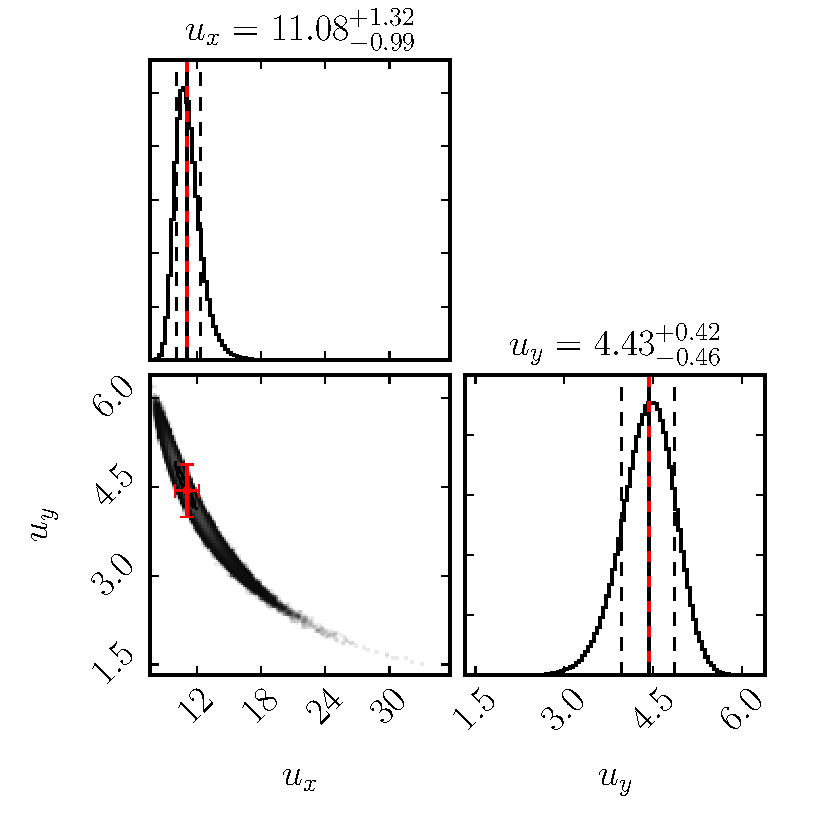
\includegraphics[keepaspectratio]{hw2_b_corner.pdf}
  \caption{The distribution of $u_y$ vs $u_x$ as well as the marginalized distributions for $u_x$ and $u_y$. The red line in the marginalized distributions shows the answer from the error propagation method, and the red point with error bars is the expected value and error from the error propagation method.}
  \label{fig:corner}
 \end{figure}
\end{enumerate}

\section{Part C}
\label{sec:partC}

\section{Part D}
\label{sec:partD}
Bayes' Theorem says
\begin{equation}
  P(A|B) = \frac{P(B|A)P(A)}{P(B)}
\end{equation}
where $P(X|Y)$ is a conditional probability of $X$ given $Y$, and $P(Z)$ is 
refered to as a \textit{prior} belief on what the value of $Z$ should be.
Frequentists equate the two conditional probabilities, but this is incorrect
in the Bayesian approach precisely because you wish to be informed by the 
priors. In this part, we assume \textit{uniform} priors on our posterior
parameters $u_x$, $u_y$ and $g$, and in addition to this there is no Jacobian 
transformation. Thus we can write for the conditional probability
\begin{align}
  \label{eq:bayesian_conditional}
  P_B(u_x,u_y,g|R,h,g) = & \frac{1}{(2\pi)^{3/2}\sigma_R\sigma_h\sigma_g} \exp\left(-\frac{(2u_xu_y/g - R_0)^2}{2\sigma_R^2}\right)\times \\ &\exp\left(-\frac{(u_y^2/2g-h_0)^2}{2\sigma_h^2}\right) \exp\left(-\frac{(g-g_0)^2}{2\sigma_g^2}\right)
\end{align}
where we have written $R$ and $h$ as functions of $u_x$, $u_y$ and $g$. Just as in class,
this expression is missing the Jacobian term,
$2u_y^2/g^2$, as calculated in \autoref{sec:partC}. Thus, if we assume flat priors
\begin{equation}
  \label{eq:priors_partD}
  P_{pr}(u_x) = P_{pr}(u_y) = 1
\end{equation}
then the ratio of the two probabilities is simply this Jacobian
\begin{equation}
  \label{eq:prob_ratio}
  \frac{P_f}{P_b} = \frac{2u_y^2}{g^2}.
\end{equation}
Interestingly, this ratio is not unitless, 
but this is not an issue since in the Bayesian 
framework we neglect the normalization terms anyway, 
which carry units with them.

We can marginalize over any two parameters to acquire the third.
See \autoref{sec:partE} for figures showing these distributions 
with no priors.

\section{Part E}
We can also introduce logarithmic priors
\begin{equation*}
  \label{eq:log_prior}
  P_{pr}(X) \propto x^{-1}
\end{equation*}
on any of our parameters. The effect is to shift (sometimes slightly)
the distributions down slightly. In the following three figures
we plot the marginalized probability for each parameter with and 
without a logarithmic prior. These probabilities were generated
by performing a numerical integral over each of the marginalized
parameters.

\begin{figure}[ht]
  \centering
  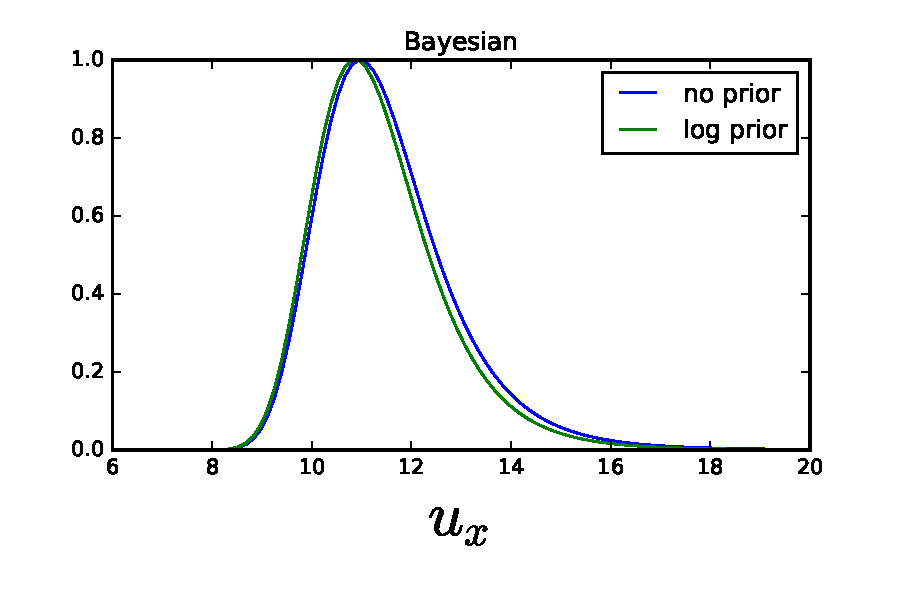
\includegraphics[keepaspectratio]{ux_bayesian.pdf}
  \caption{The marginalized probability of $u_X$. The marginalization
    over the other two parameters was done numerically.}
  \label{fig:ux_bayesian}
\end{figure}

\begin{figure}[ht]
  \centering
  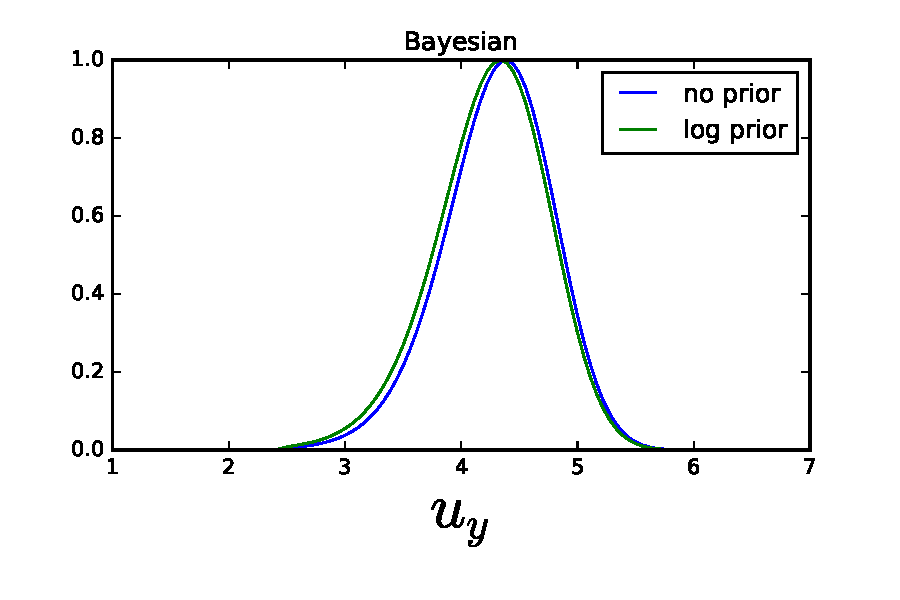
\includegraphics[keepaspectratio]{uy_bayesian.pdf}
  \caption{The marginalized probability of $u_y$. The marginalization
    over the other two parameters was done numerically, however
    one may perform the marginalization over $u_x$ analytically in
    this exercise.}
  \label{fig:uy_bayesian}
\end{figure}

\begin{figure}[ht]
  \centering
  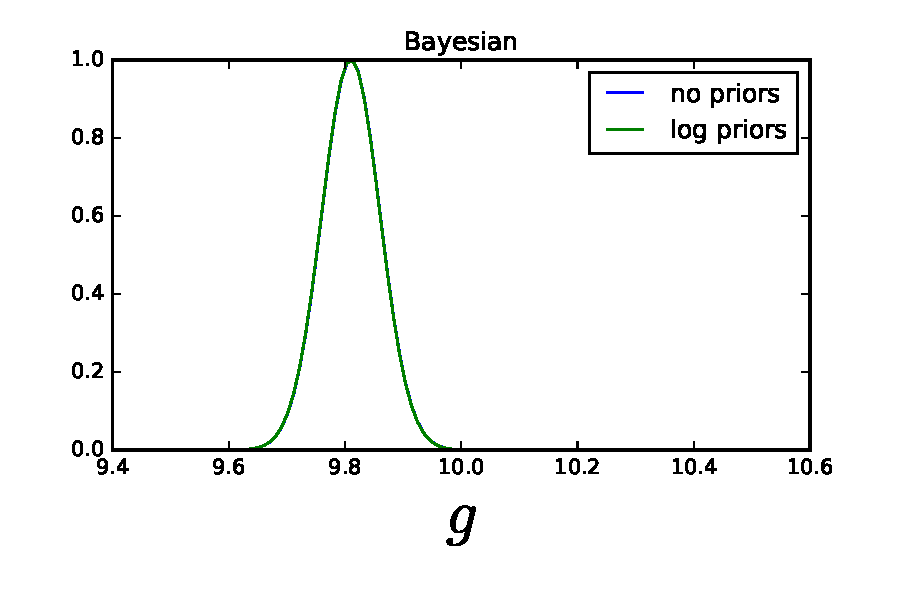
\includegraphics[keepaspectratio]{g_bayesian.pdf}
  \caption{The marginalized probability of $g$. The marginalization
    over the other two parameters was done numerically, however
    one may perform the marginalization over $u_x$ analytically in
    this exercise.}
  \label{fig:g_bayesian}
\end{figure}





\newpage

\section*{References}

\end{document}
